
\section{Naive Bayes Classifier}
In this section we chose the task of classifying songs' emotion using the Naive Bayes classifier. The classifier solved a binary classification, through which a track was labeled either as "happy" or "sad".
The labels were engineered starting from the attribute \textit{"valence"} provided in \textit{"echonest.csv"}. \textit{"Valence"} is an attribute that has a range that goes from 0 to 1 (generated by Echo Nest using internal algorithms). The highest this value is, the more a given track transmits to the user positive vibrations. We set a threshold of 0.55, so that songs with a valence score lower than the threshold were labeled as sad songs while the others as happy. The classes are almost balanced, although the majority of tracks are sad songs. The partition is the following: 7,724 "sad" and 5,405 "happy" songs, for a total of 13,129 records. The features used for training the Naive Bayes classifier are: \textit{acousticness, danceability, energy, instrumentalness, liveness, speechiness, tempo}. 
Their choice is driven by the fact that they shown low correlation(Figure 3.1), which is essential for the independence assumption made by the Naive Bayes Classifier. We performed a binary label encoding and split the data into training (70\%) and test set (30\%). We didn't apply a normalization, as it doesn't affect the way probabilities are estimated. 

\begin{figure}[!htb]
  \centering
  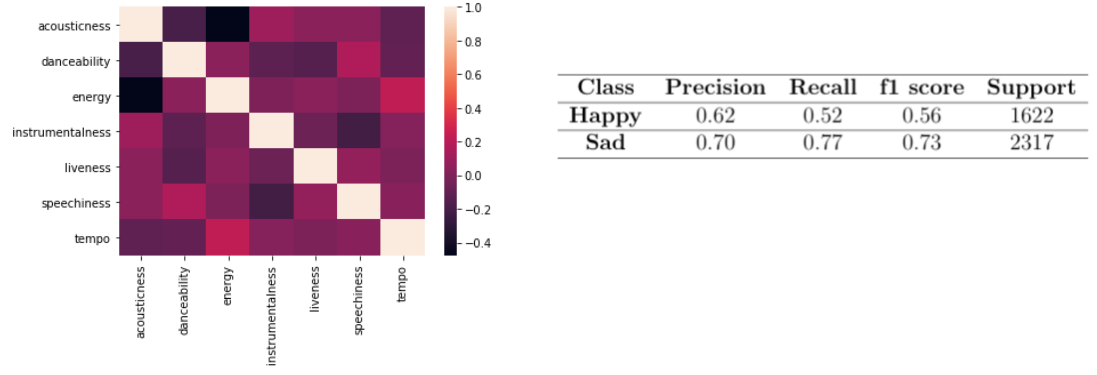
\includegraphics[width=0.85\linewidth]{images/corr-matrix_scores-naivebayes-classif-report.png}
  \caption{On the left the Correlation Matrix of features used in the Naive Bayes. On the right the Classification Report. }
\end{figure}

\begin{figure}[!htb]
  \centering
  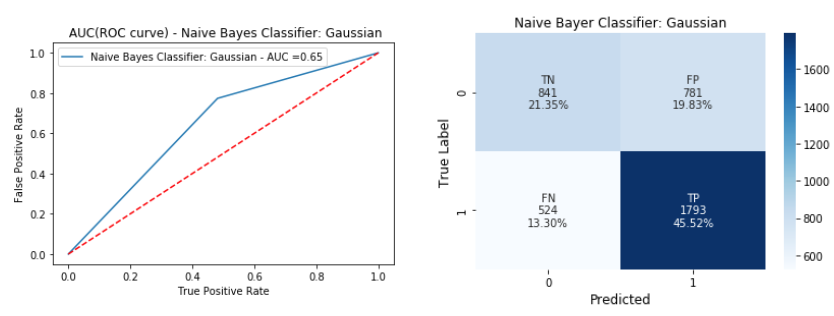
\includegraphics[width=0.7\linewidth]{images/ROC-CFM-Naive-Bayes.png}
  \caption{ROC curve and Confusion Matrix of Gaussian Naive Bayes.}
\end{figure}

Overall the model performed discretely with an accuracy of 67\%. It is interesting to see that the model had better performance in predicting the class "sad". Furthermore, the number of False positive is quite high. In fact the classifier labeled as "sad" almost half of the happy songs present in the dataset (which explains the recall of 0.52).

\section{Multi-Layer Perceptron}
In this section we constructed a Multi-Layer Perceptron for solving the same task described in the previous section (songs' emotion recognition). 
\subsection{Data Preparation}
The dataset chosen for this binary-task is \textit{features.csv}, which counts of 13,129 input patterns and 518 features.  As emotions are usually associated to the tonality and pitch of a song, we considered the attributes provided by \textit{features.csv} more suitable than the ones of \textit{echonest.csv} to train a Neural Network. We detached the labels from the dataset and we encoded them into binary values. Lastly, we normalized the dataset paying attention to don't bias the development set with information regarding the distribution of the test set.
\subsection{Validation Schema \& hyper-parameters tuning}
The data was split into \textbf{development set} and \textbf{test set}, using a split ratio of 30\%. The split was stratified, so to assure that the data in each partition represented the same proportion of the class.
The test set was never used during the model selection and training phase, to assure an unbiased estimation. 
The development set was further split into \textbf{training set} and \textbf{internal test set}. The training set was used exclusively for model selection, whereas the internal test set was used to evaluate the performance and compare models. In Table 3.1 we report the data partitions. 

% Data partitions MLP
\begin{table}[!htb]
\centering
\begin{tabular}{ccc}
\hline
\multicolumn{2}{c}{\textbf{Development set}}       & \textbf{}         \\ \hline
\textbf{Training set} & \textbf{Internal Test set} & \textbf{Test set} \\
6433                  & 2757                       &     3939              \\ \hline
\end{tabular}
\caption{Data partitions.}
\label{Data partitions}
\end{table}
In order to find the right hyper-parameters' setting, we first tried different configuration so to get an initial idea of what architecture and parameters worked best for the task at hand. We then performed a coarse-to-fine random search using a \textbf{5 fold cross validation}.\\ 
The optimal configuration found by the coarse search, was given in input to a randomized grid search which tested random configuration of hyper-parameter within the range of the parameters discovered in the coarse phase. Different models were compared using the internal test set as internal performance estimator. In order to reduce the size of the hypothesis space, we used only the binary cross entropy for training the model. In Table 3.2 we show the coarse configurations used in the randomized grid search. 

% Parameters' search - MLP
\begin{table}[h]
\centering
\resizebox{\textwidth}{!}{%
\begin{tabular}{ccclll}
\hline
\textbf{Hidden Layers}                                                                                                     & \textbf{Learning rate}                                                   & \textbf{Solver} & \textbf{Momentum}                                                & \textbf{lambda}                                                                    & \textbf{Activations} \\ \hline
\begin{tabular}[c]{@{}c@{}}{(50,), (50,50), (50, 50, 50),\\ (60,20), (20, 20, 20 ,20), \\ (100,), (100, 20) }\end{tabular} & \begin{tabular}[c]{@{}c@{}}{0.1, 1e-1, 1e-2,\\  1e-3, 1e-4}\end{tabular} & {Adam, SGD}     & \begin{tabular}[c]{@{}l@{}}{None, 0.2, \\ 0.5, 0.8}\end{tabular} & \begin{tabular}[c]{@{}l@{}}{None, 1e-1, \\ 1e-2, 1e-3, \\ 1e-4, 1e-5}\end{tabular} & {Sigmoid, ReLU}      \\ \hline
\end{tabular}%
}

\caption{Hyper-parameters used in the corase randomized grid search. The lambda refers to the Tikhonov regularization coefficient. It's important to notice that the activation function of the output layer is not tested in the randomized grid search. Since we solved a binary classification task, the output activation function was set to be a Sigmoid.}
\label{Hyperparameters coarse randomized search}
\end{table}

The best model resulted to be the one with 2 hidden layers of 60 and 20 neurons each. Below we show the configuration of the best model. 

% Model Architecture Best model MLP
\begin{table}[!htb]
\centering
\resizebox{\textwidth}{!}{%
\begin{tabular}{ccclll}
\multicolumn{6}{c}{\textbf{Model's Architecture}}                                                                                    \\ \hline
\textbf{Hidden Layers} & \textbf{Learning rate} & \textbf{Solver} & \textbf{Momentum} & \textbf{lambda} & \textbf{Activations}     \\ \hline
(60,20)                & 0.00112                & SGD             & 0.7934            & 0.11744         & \multicolumn{1}{c}{ReLU} \\ \hline
\end{tabular}%
}
\caption{Architecture of the best model}
\label{Architecture of the best model}
\end{table}

\subsection{Analysing overfitting effects}
When selecting the best model, we carefully inspected the loss curves of training and validation so to detect possible overfitting. We noticed that given the high number of features (518) and sub-sequentially the high number of free parameters, the model was prone to overfitting. However, the right regularization coefficient was helpful in controlling the complexity of the model and avoid overfitting. 
In Figure 3.3 we compare the models with and without regularization.

The loss curves for training and validation are stable and are not diverging for the model with regularization. This is a clear indicator that the model is not overfitting the data. The accuracy on the validation set is 77.53\%, which is considered a good result considering the task we are attempting to solve. The model on the right instead (the one without regularization) shows a validation curve that starts to increase after 300 epochs, while the training curve decreases to 0. To get an estimate of the model performances on previously unseen data, we tested it on an internal test set. The accuracy on the final test was expected to be approximately 75.98\%. 

\begin{figure}[h]
  \centering
  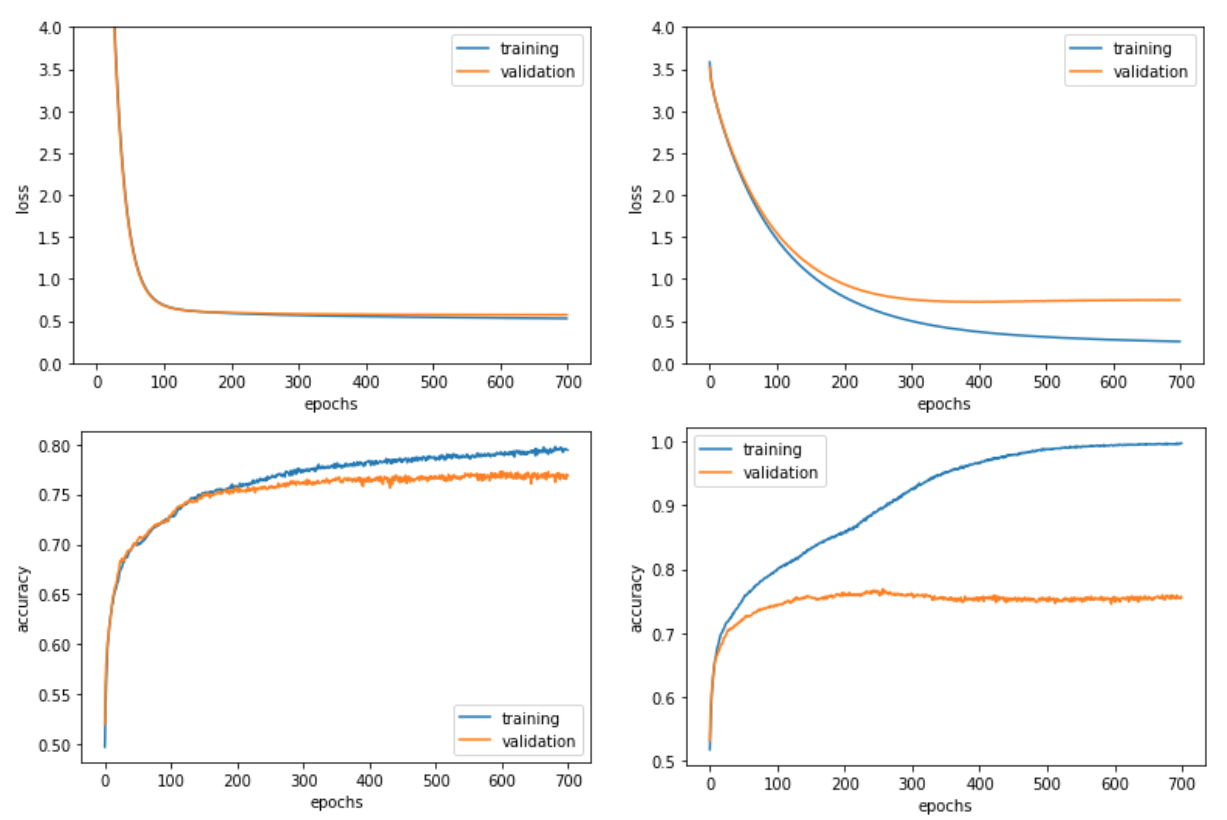
\includegraphics[width=0.6\linewidth]{images/MLP loss-acc comparison .png}
  \caption{On the left we show the loss (binary cross-entropy) and accuracy of the model with regularization. On the right the loss (binary cross-entropy) and accuracy of the model without regularization.}
\end{figure}

\subsection{Final Evaluation}
The best model was retrained on the full development set (training set + internal test set) and then tested on the test set. Below we show the classification report along with the confusion matrix and ROC curve.
The accuracy on the test set is 75.72\% which is close to the one estimated on the validation set. Analyzing the intra-class scores, we observe that the precision recall and f1 score are high for both classes, although the model can detect sad songs with higher precision (80\%). Overall the model was able to capture and learn the features needed for detecting emotions in a song. 

\begin{figure}[!htb]
  \centering
  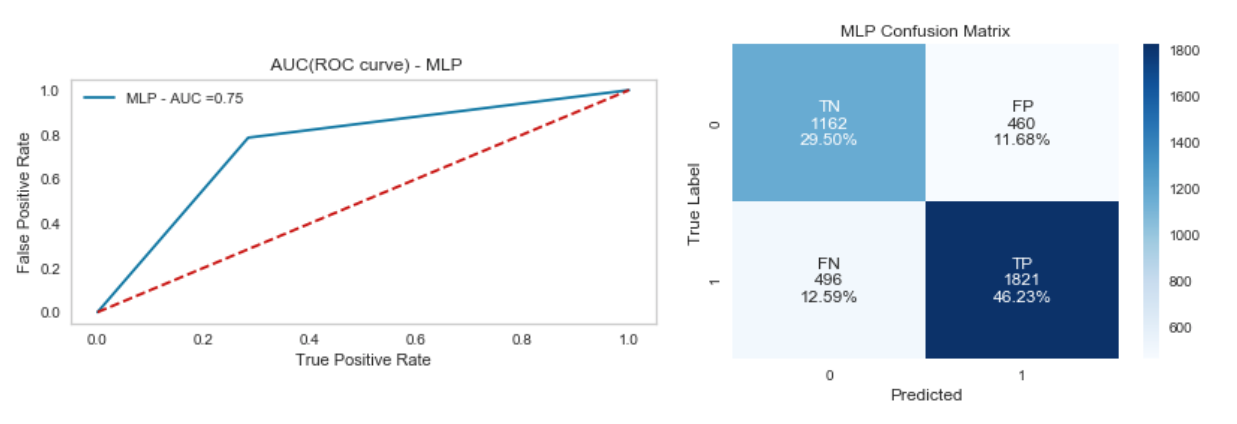
\includegraphics[width=0.7\linewidth]{images/MLP-confusion-matrix_ROC-curve_.png}
  \caption{Confusion Matrix and ROC curve of MLP.}
\end{figure}


\begin{table}[!htb]
\centering
\begin{tabular}{ccccc}
\hline
\textbf{Class} & \textbf{Precision} & \textbf{Recall} & \textbf{F1} & \textbf{Support} \\ \hline
Happy          & 0.70               & 0.72            & 0.71        & 1622             \\ \hline
Sad            & 0.80               & 0.79            & 0.79        & 2317            
\end{tabular}
\caption{Classification report: Test set MLP.\\ Accuracy = 75.72\%. }
\label{Classification report: Test set Linear SVM}
\end{table}







\section{Support Vector Machines}
In this section we experimented with linear and non-linear support vector machines for the task of Song emotion recognition. This binary classifier was able to detect sadness and happiness of a song.
The attributes employed are the ones provided in \textit{"features.csv"}.

\subsection{Data Preparation \& Validation Schema}
The data was normalized using a standard scaler, while the labels were encoded into binary values.  The data was partitioned in training set (70\%) and test set (30\%). 
The optimal hyper-parameters were obtained performing a random search in a combination with a 5 fold cross validation. We tested 300 configurations for each model (Linear and Non-Linear SVM), whose parameters were randomly generated from a uniform distribution.


\subsection{Linear SVM}
The optimal setting for the C parameter is 0.4329, which provided us an accuracy on the validation set of 74.61\%. The performance on the test set instead was higher than our estimation. In fact the model reported an accuracy of 76\%. The recall for both classes is quite balanced (78\% sad and 75\% happy). However the precision on the class sad songs is much higher than the one of happy songs ( 83\% and 68\% respectively). The AUC score instead, is approximately 76\%. 

\begin{table}[!htb]
\centering
\begin{tabular}{ccccc}
\hline
\textbf{Class} & \textbf{Precision} & \textbf{Recall} & \textbf{F1} & \textbf{Support} \\ \hline
Happy          & 0.68               & 0.78            & 0.73        & 1622             \\ \hline
Sad            & 0.83               & 0.75            & 0.79        & 2317            
\end{tabular}
\caption{Classification report: Test set Linear SVM.\\ Accuracy = 76\%. }
\label{Classification report: Test set Linear SVM}
\end{table}

\subsection{Non-Linear SVM}
The SVM with non-linearity was tested using several kernels( RBF, polynomial, linear and Sigmoid) and C configurations. The best model resulted to be the one with the RBF kernel and a C = 1.419. It's important to mention that the performance with the other kernels were quite low and didn't reach more than 67\% accuracy. 
With RBF kernel instead, we reached an accuracy on the test set of 77\% (1\% higher than the one obtained with linear SVM). The non-linearity introduced by the kernel, allowed us to improve the precision of the class Happy (which is now 74\% against the 0.64\% of linear SVM). The boost in performance is also noticeable in the f1 score of class sad songs (now 81\%).
Lastly, we didn't noticed substantial changes in the AUC score (which is still 76\%). 
\\
\begin{table}[!htb]
\centering
\begin{tabular}{ccccc}
\hline
\textbf{Class} & \textbf{Precision} & \textbf{Recall} & \textbf{F1} & \textbf{Support} \\ \hline
Happy          & 0.74               & 0.70            & 0.72        & 1622             \\ \hline
Sad            & 0.80               & 0.82            & 0.81        & 2317            
\end{tabular}
\caption{Classification report: Test set Non-Linear SVM.\\ Accuracy = 77\%. }
\label{Classification report: Test set Non-Linear SVM}
\end{table}

\subsection{Final Evaluation}
Comparing the two models, we observe that apart from the improvement in the accuracy, the non-linear SVM increased the True Positive ratio(48.71\% against 44.02\%) and diminished the number of False Negatives down to 10.31\%. Although similar, non-linear SVM resulted to be the best model. 

\begin{figure}[!htb]
  \centering
  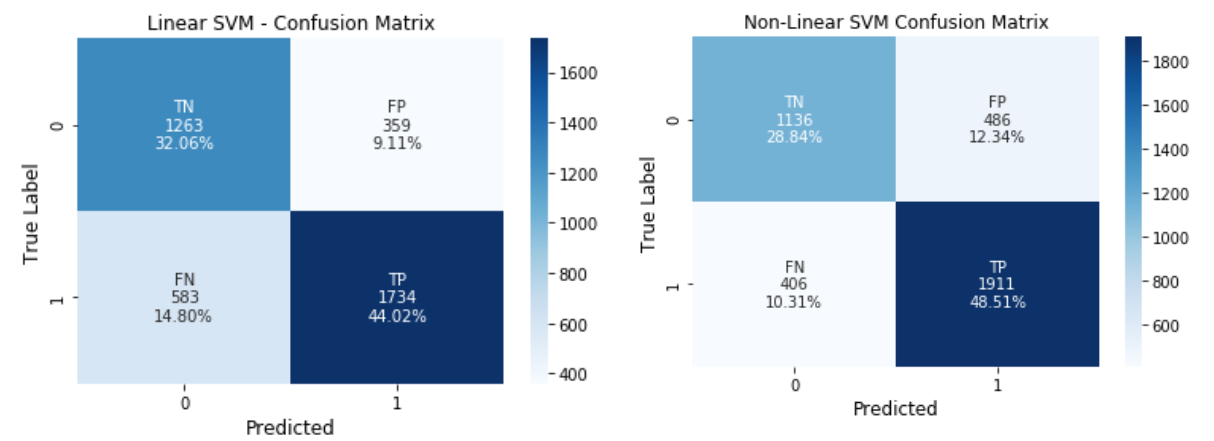
\includegraphics[width=0.7\linewidth]{images/Confusion_matrix-Linear-NonLinear-SVM.png}
  \caption{Confusion matrix for SVM with Hard Margin and SVM with Soft Margin.}
\end{figure}

\section{Rule based classifiers: RIPPER algorithm}

We employed the RIPPER rule-based classifier, for solving the binary classification task: Electronic - Classical. 
The task we proposed to solve was not of high complexity (the classes were well separated), as the two genres are noticeably different one from one another. However the dataset presents an high class imbalanced, which do not affect the RIPPER algorithm, as the latter is suitable for classifying instances of unbalanced datasets. The features used to train the models were extracted from the partition of \textit{"echonest audio\_features"}(\textit{acousticness, danceability, energy, instrumentalness, liveness, speechiness, tempo, duration} and \textit{bit\_rate}). Before growing the rules required for classifying the test-data, we removed the top 1\% of outliers (using the techniques described in chapter 2) and made sure that the dataset didn't have missing or duplicate values. The dataset consisted of 2,288 tracks. Electronic songs represented 90.51\% (2,071 rows) of the data, while Classical 9.48\% (717 rows).
The rule-set was grown by setting the majority class (Electronic) as default class and learn rules on the positive class (Classical). In order to maximize the results, we tested the performance of the model using different prune sizes. The latter ranged from 0.2 to 1. 
The highest performances were provided when the prune size was set to 0.5. As this increased the model was not able to discriminate the class labels. On this task, RIPPER performed exceptionally, obtaining an AUC score of 94\% and a recall on the minority class of 90\%.

\begin{figure}[!htb]
   \begin{minipage}{0.46\textwidth}
     \begin{tabular}{ccccc}
     \hline
     \textbf{Class} & \textbf{Precision} & \textbf{Recall} & \textbf{F1} & \textbf{Support} \\ \hline
     Electronic          & 0.99               & 0.98            & 0.98        & 622             \\ \hline
     Classical            & 0.81               & 0.90            & 0.85        & 65            
     \end{tabular}
     \caption{Classification report: Test set RIPPER. Accuracy = 97\%. }
     \label{Classification report: Test set Ripper}
   \end{minipage}\hfill
   \begin{minipage}{0.42\textwidth}
     \centering
     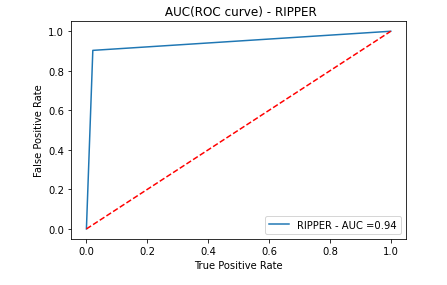
\includegraphics[width=1\linewidth]{images/auc-ripper.png}
     \caption{ROC curve - RIPPER}\label{Fig:Data2}
   \end{minipage}
\end{figure}


\begin{figure}[!htb]
  \centering
  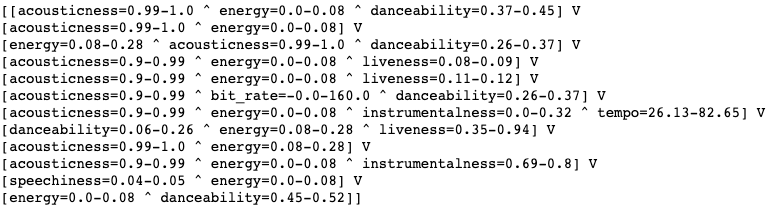
\includegraphics[width=0.75\linewidth]{images/ruleset-out_model.png}
  \caption{Ruleset extracted on the positive class. For better readability the symbol \^\ can be read as \textbf{AND} while V as \textbf{OR}.}
\end{figure}

In Figure 3.8, we show the rules learned on the positive class. It is interesting to notice that the majority of the rules in the decision list, have conditions on the variables \textit{"acousticness"} (present in almost 66\% of the rules) and \textit{"energy"}, whose appear to be determinant in classifying classical songs. Observing the rules, classical song has high acousticness(0.9 to 1) and low energy (usually in range 0 - 0.08). 



\section{Linear Regression}
In this section we built a Linear Regression model able to predict the variable \textit{"danceability"} using \textit{"valance"} as independent variable. To achieve this, we filtered the dataset by considering only one genre at the time. The choice is driven by the fact that if we considered the genres all together, the linear correlations would have been hidden due to genres' diversity. The highest linear correlation between the dependent and independent variable was provided by the genre Historical and Jazz, for which the correlation is +0.61 and +0.5.

\subsection{Data Preparation}
The dataset for Historical has 349 tracks, while the one for Jazz counts 233 records. Before constructing the model we removed 1\% of the outliers, as they could have negatively influenced the computation of the hyper-parameters of the regression line. Ultimately, the datasets were split into training set (70\%) and test set(30\%). We also checked if introducing a regularization terms improved the fit of the regressor ( we tested Ridge and Lasso regularizations). The parameter $\alpha$ (penalty term) was tuned using a randomized grid search and 5 fold cross validation (we tested values in range $[10^{-6},1]$).

\subsection{Simple Linear Regression}
The best fit was obtained on the dataset of Historical tracks without regularization. Analyzing the $R^2$ score, we could notice that the variable \textit{"valence"} is able to predict almost 51\% of the variance of the dependent variable \textit{"danceability"}. 
The same score however, decreased when introducing a regularization. The model has a MSE of 0.011 on the test set (the MAE is 0.087). 
The model without regularization, has a better fit also on the Jazz dataset. The $R^2$ is 0.320, while the MSE is 0.017. 


\begin{figure}[!htb]
  \centering
  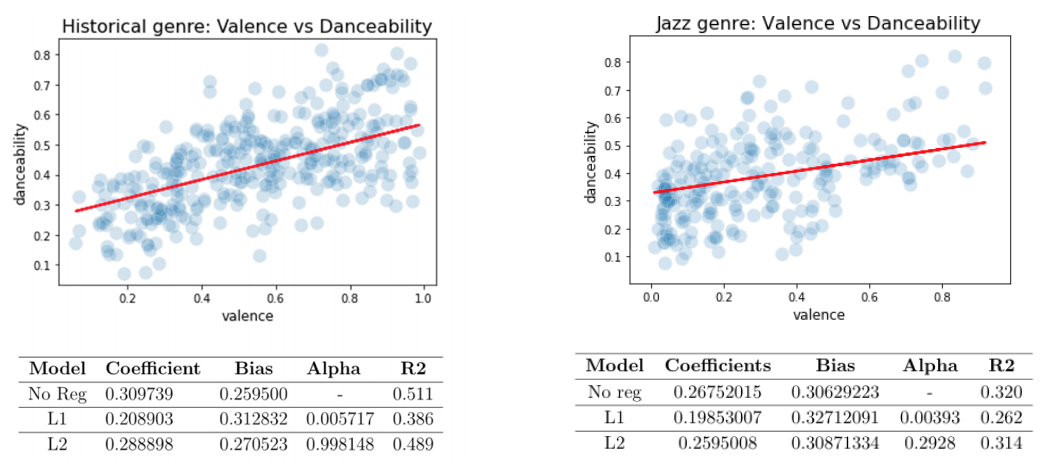
\includegraphics[width=1\linewidth]{images/lr-functions-tables.png}
  \caption{From left to right we show the scatter-plots of the models with the best fit (on Historical and Jazz dataset). Below the graphs we show the results obtained on each model.}
\end{figure}


\subsection{Multiple Linear Regression}
We attempted to improve the performance of the linear regression model constructed for predicting the variable \textit{"danceability"} of the "Historical" genre, by increasing the number of independent variables.
The variables chosen for building a multiple linear regression model, were \textit{"energy"} and \textit{"speechiness"}. These additional variables are those which had the second and third highest correlation with the dependent variable (the others had negative or zero correlation). 
The best multiple liner regressor is the one without regularization, in fact the $R^2$ for this model is 0.509 (slightly lower than the one obtained with the linear regression). The MSE for the model without regularization is 0.011. The latter increases if we increment the variable "alpha", meaning the regularization is slightly causing our model to underfit the data. Overall, we noticed that w.r.t the linear regressor, the multiple linear regressor didn't improve the performance. This is probably due to the fact that the additional variables were not strongly correlated with the dependent one.

\begin{figure}[!htb]
  \centering
  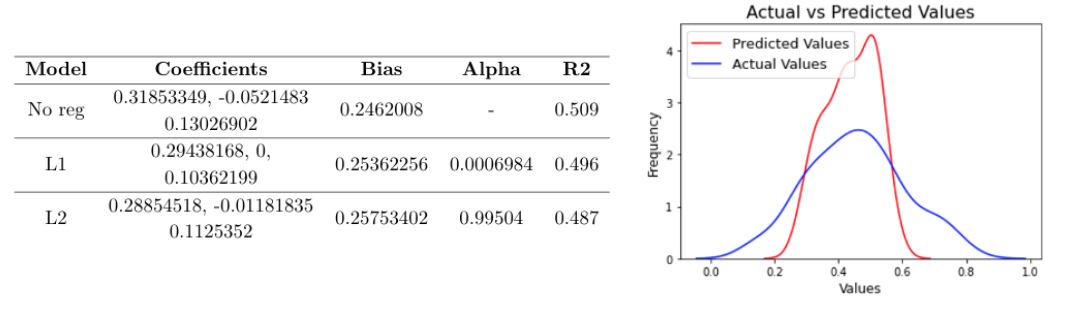
\includegraphics[width=1\linewidth]{images/mlr-act-pred-tab-hist.png}
  \caption{On the left we show a table summarizing the parameters of the model and the $R^2$ score. On the right we show the distribution of the predicted/actual values and their frequency. We can observe that using the regression line, we are predicting with more frequency values ranging approximately from 0.4 to 0.6.  
  }
\end{figure}

%%%%%%%%%%%%%%%%%%%%%%%%%%%%%%%%%%%%%%%%%%%%%%%%%%%%%%%%%%%%%%%%%%%%%%
\newpage
\section{Logistic Regression}
In this section we employed a Logistic Regression to classify songs' emotion. In order to solve this binary task we chose the following features: \textit{acousticness, danceability, energy, instrumentalness, liveness, speechiness, tempo, duration} and \textit{bit\_rate}. 

\subsection{Data Preparation \& Analysis}

The dataset containing 13,129 rows (7,724 sad and 5,405 happy songs) was split into training set(70\%) and test set(\%). The labels were encoded in binary variables and the features were normalized using a standard scaler. Before deploying the model, by means of a recursive feature selection, we checked if by removing attributes, the accuracy on the validation set increased. We noticed that the highest results were obtained when all features were utilized, hence we proceeded using all attributes available. 
\subsection{Model Evaluation}
If we analyze the classification report we notice that even though the precision is lower for class "happy" (56\% compared to 76\% of class "sad"), the model is able to identify 71\% of happy songs(as shown by the recall). Since the classes are not highly unbalanced, we considered the accuracy as a good performance estimator. The score obtained on the test set is 68\% which is considerably low compared to the one obtained by the models described in the previous sections (for the same task). In Figure 3.12, we can observe that the strongest feature is \textit{"danceability"}, which has an higher importance (+0.10) compared to the others.

\begin{figure}[!htb]
   \begin{minipage}{0.46\textwidth}
     \begin{tabular}{ccccc}
     \hline
     \textbf{Class} & \textbf{Precision} & \textbf{Recall} & \textbf{F1} & \textbf{Support} \\ \hline
     Happy          & 0.59               & 0.71            & 0.65        & 1622             \\ \hline
     Sad            & 0.76               & 0.66            & 0.71        & 2317            
     \end{tabular}
     \caption{Classification Report Logistic Regression - Songs' emotion.
Accuracy = 68\%.}
     \label{Classification report: Test set Ripper}
   \end{minipage}\hfill
   \begin{minipage}{0.42\textwidth}
     \centering
     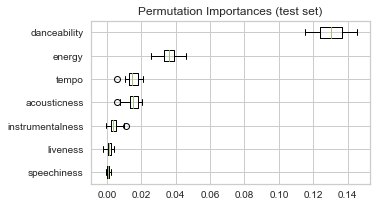
\includegraphics[width=1\linewidth]{images/perm log-reg.png}
     \caption{Features permutation of Logistic Regression run over 20 trials.}\label{Fig:Data2}
   \end{minipage}
\end{figure}
\newpage
The confusion matrix highlights the fact that the False Positive and False Negative are quite high. In fact we noticed that 20.11\% of "happy" songs, were wrongly predicted as "sad", while it misclassified only 11.98\% of "sad". The AUC score instead is 68\%, which is almost 10\% lower than the score obtained using other models. 


\begin{figure}[h]
  \centering
  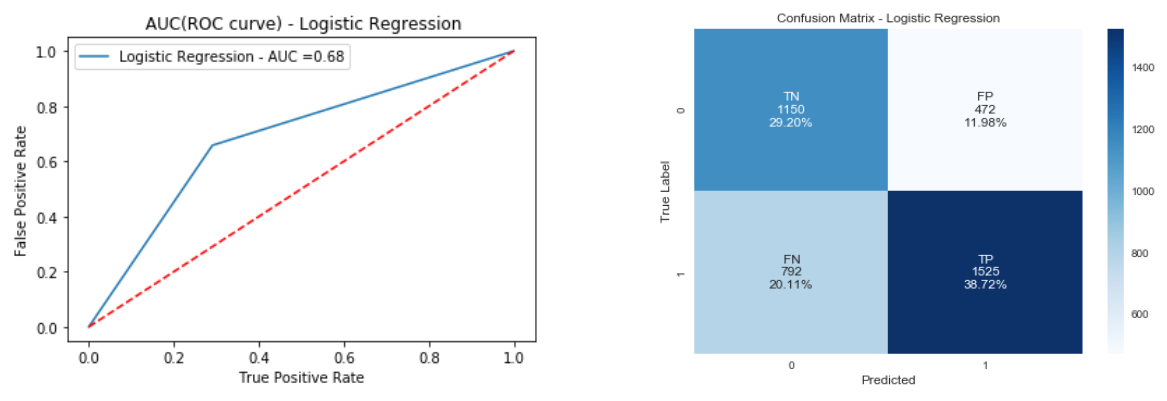
\includegraphics[width=0.74\linewidth]{images/log-reg_ROC-CFM.png}
  \caption{On the right the ROC curve, while on the left we show the Confusion Matrix of the Logistic Regression.
  }
\end{figure}


%%%%%%%%%%%%%%%%%%%%%%%%%%%%%%%%%%


\section{Ensemble methods}
Ensemble classifiers were built for classifying songs' emotion. The dataset used for the classification task is \textit{"features.csv"}. 
We also report an experimental evaluation of a single decision tree (base estimator) which was used as a benchmark to compare different ensemble techniques. Its hyper-parameters were fine tuned through a random search in combination with a 5 fold cross validation, which tested 400 configurations and returned the one with the highest accuracy on the validation set. Our aim was to improve the performance of the base classifier using ensemble techniques. In Table 3.7 we show the classification report of a single decision tree. 
 
\begin{table}[!htb]
\centering
\begin{tabular}{ccccc}
\hline
\textbf{Class} & \textbf{Precision} & \textbf{Recall} & \textbf{F1}   & \textbf{Support} \\ \hline
Happy & 0.70      & 0.67   & 0.63 & 1622    \\ \hline
Sad   & 0.75      & 0.69   & 0.72 & 2317    \\
\end{tabular}
\caption{Classification report of base estimator:  Decision Tree.\\ 
Accuracy: 68\%}
\label{Classification report: Decision Tree Ensemble}
\end{table}


\subsection{Random Forest}
The random forest was built taking into account the performance of models constructed with different number of estimators. The base estimator of the forest was the single (optimized) decision tree described above. The optimal random forest employed 200 estimators for classifying samples as "happy" or "sad". As it emerges from the features permutation (run over 10 trials), the most significant feature was \textit{"tonnetz"}. 
In terms of performance, the model was able to correctly predict only 50\% of class "happy", with a precision of 71\%. The scores reported for the latter, are definitely inferior w.r.t. those of class "sad". We noticed that even though the overall accuracy increased of +3\%, the ability of recognizing "happy" song diminished when using a random forest. Substantial improvements were obtained on the recall and f1 score of class "sad", which were 86\% and 78\% respectively (as we can see in Figure 3.14).

\begin{figure}[!htb]
   \begin{minipage}{0.45\textwidth}
     \begin{tabular}{lllll}
        \hline
        \textbf{Class} & \textbf{Precision} & \textbf{Recall} & \textbf{f1 score} & \textbf{Support} \\ \hline
        Happy          & 0.71               & 0.50            & 0.59              & 1622             \\ \hline
        Sad            & 0.71               & 0.86            & 0.78              & 2317            
     \end{tabular}
     \caption{Classification report - test set: Random Forest with 200 estimators.\\ Accuracy: 71\%}
    \label{Classification report: Random Forest}
   \end{minipage}\hfill
   \begin{minipage}{0.47\textwidth}
     \centering
     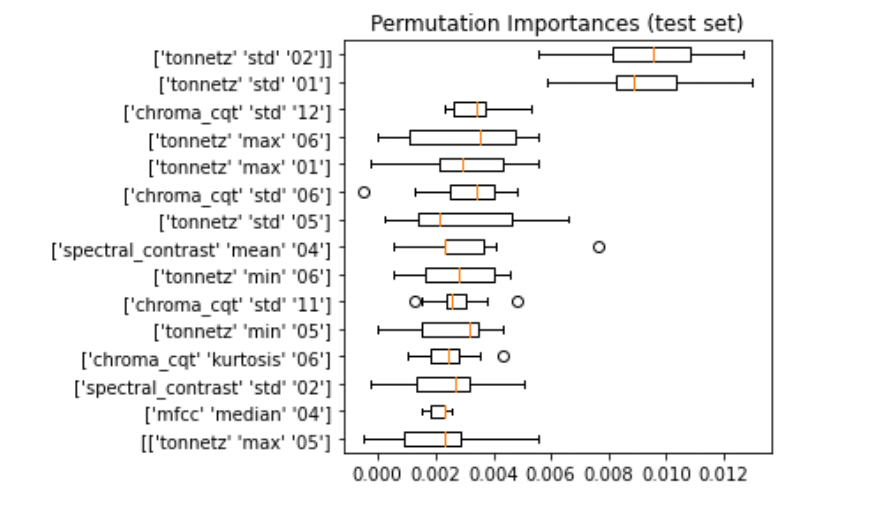
\includegraphics[width=1\linewidth]{images/rf_permutation-importance.png}
     \caption{Features permutation.}
   \end{minipage}
\end{figure}


\subsubsection{Performances varying number of estimators}

We observed how the model behaved when we varied the number of estimators. The number of configurations that were tested are: 50, 100, 200, 400 and 800. We noticed that the accuracy of the classifier did not exceed 70\% when the estimators were ranging from 50 to 100. In general increasing the estimators, improved the scores of class "happy" (i.e. with 50 estimators the f1 score was 58\%, while it increased up to 59\% when we added trees to the forest). For our model, 200 estimators resulted to be the "sweet-spot", as it improved the accuracy (71\%) as well as the recall of class "happy". When the number of estimators were raised from 200 to 800, the overall performance appeared to converge, as we did not notice any significant gains. 



\subsection{Bagging}

Noticeable improvements were provided by bagging. In terms of accuracy we noticed an increase of +1\% (72\% accuracy) w.r.t. random forest. The recall of class "happy" did not reach a score higher than 59\% (which is still a better result than the one provided by random forest). We recorded a clear betterment in the f1 score of class "happy" and in the precision of class "sad" (74\% against 71\% of random forest). 

\begin{table}[!htb]
\centering
\begin{tabular}{lllll}
\hline
\textbf{Class} & \textbf{Precision} & \textbf{Recall} & \textbf{f1 score} & \textbf{Support} \\ \hline
Happy & 0.68      & 0.59   & 0.63     & 1622    \\ \hline
Sad   & 0.74      & 0.81   & 0.77     & 2317   
\end{tabular}
\caption{Classification report - test set: Bagging Decision Tree.\\ 
Accuracy: 72\%}
\label{Classification report: Bagging Decision Tree}
\end{table}


\subsection{Adaboost}
Adaboost is known for providing improvement in the performance of classifiers built for solving even the most difficult task. The principles exploited by this algorithm proved to be effective also in our case. In fact this ensemble method is the one that significantly "boosted" the accuracy of the model. To build the ensemble we used 400 stumps (tree with depth = 1). We noticed that as we increased the depth of the trees, the ensemble was more prone to overfitting the training data. When using stamps, the accuracy estimated on the validation set is 72.6\% (training accuracy = 75.89\%). The expected score almost matched the one obtained on the test test (73\%). The ensamble improved the f1 score of class "happy" (67\% against 63\% of the decision tree used as a benchmark). Important improvement were also observed for the recall and precision of both classes. The classification report is shown in Table 3.9.  

\begin{table}[!htb]
\centering
\begin{tabular}{lllll}
\hline
\textbf{Class} & \textbf{Precision} & \textbf{Recall} & \textbf{f1 score} & \textbf{Support} \\ \hline
Happy & 0.68      & 0.67   & 0.67     & 1622    \\ \hline
Sad   & 0.77      & 0.78   & 0.77     & 2317   
\end{tabular}
\caption{Classification report - test set: AdaBoost.\\Accuracy: 73\%}
\label{Classification report: AdaBoost}
\end{table}

\subsection{Comparing Ensembles Techniques}

\

All the ensemble methods that were tested, improved the performance of the single decision tree. Ensembles proved to be a powerful tool for refining the accuracy of our classifier. Among those that were analyzed, Adaboost was the one with the highest scores. The AUC observed for this method is 80.3\% (+6.5\% w.r.t. a single decision tree). Random forest and bagging have almost equal performances, as the AUC difference is minimal.   

\begin{figure}[htb!]
  \centering
  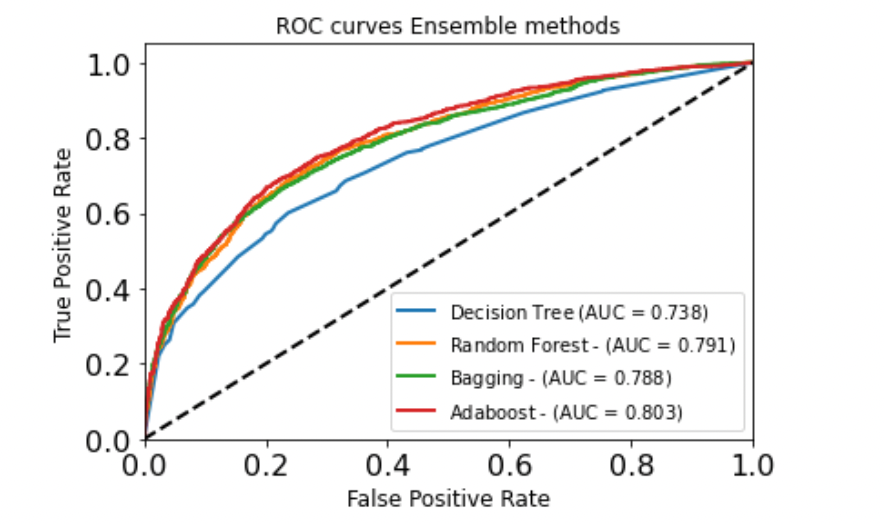
\includegraphics[width=0.5\linewidth]{images/ensemble-classifiers.png}
  \caption{ROC curves ensemble. }
\end{figure}
\section{Impact of Different Data Sizes}

In this section we analyzed how different amount of training data, affected the performances of the following classifiers: SVM, Multi-Layer Perceptron(MLP), Decision Tree(DT), KNN and Random Forest. The models were tested on the dataset \textit{"features.csv"} for solving the task of songs' emotion classification. Each model was tested on different percentages of training data. Ultimately, we compared their performances in terms of accuracy (as shown in Figure 3.17).
We notice that SVM has the highest performaces, with a trend that grows almost linearly w.r.t. the increasing size of the training data. Random Forest has better performances than the MLP until the size of the training data exceeds 50\%. In fact from that point on, the MLP is the second model with the highest accuracy (72.5\%). The accuracy of the DT is negatively affected when the data passes from 40\% to 50\% (the accuracy decreases of 2.5\%), while the KNN seems to start gaining better accuracy as we add records to the training data.

\begin{figure}[htb!]
  \centering
  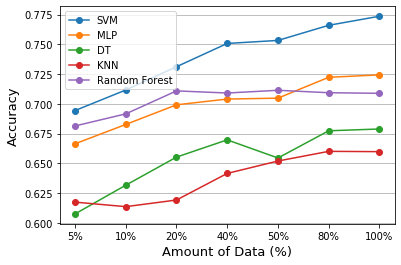
\includegraphics[width=0.4\linewidth]{images/models-comparision-different-training-sizes.png}
  \caption{Performances in terms of accuracy for models trained on different subsets of training data.}
\end{figure}